%%% The first section of your paper. 

\section{Introduction}

Contemporary Product Design process heavily depends on CAD applications. They present easy-to-use ways for defining models, attributes, relationships etc.  These models can then be used in associated domains like drafting, analysis, manufacturing etc. Many commercial CAD applications use {\em Design-by-Features} paradigm. {\em Features}, not only embed meta-information based on application's need  but also carry shape information (geometry, topology)  \cite{Brunetti2003}. {\em Features} also reflect vocabulary used in the particular domain making them intuitive to use. Such proliferation of {\em Features} has led to various {\em feature-schema} not only in different CAD applications but also in different modes of the same CAD application. In a particular application, different features may generate same Shape, e.g. {\em features} like {\em Box}, {\em Pad}, {\em Protrusion}, {\em Extrude}, which presented differently, represent the same shape. Such diversity has created problems in learning a CAD system, interoperability between CAD applications, and also in the development of algorithms for domains like, Computer-Aided-Manufacturing (CAM) and Computer-Aided-Engineering (CAE). This can be seen in relatively lesser usage of {\em features} in those applications, especially CAE.  One of the solutions could be to come up with a neutral way of defining {\em form features} so that once algorithms are based on that neutral definition; they can be implemented in variety of CAD-CAE applications. 

This paper proposes an abstraction scheme of {\em form features}, their notation in terms of Spatial Grammars and also its use in a generic way for {\em Midsurface} algorithm in CAE. This proposed approach has potential to address interoperability and portability issues in CAD applications.

\section{Related Work}

	Following sections explore major contributions in the areas relevant to topics, like, Spatial Grammars, Feature Representation, Midsurface Representation and Generic Programming.

\subsection{Spatial Grammars}

Spatial Grammars encompasses representation schema such as Graph Grammars, Shape Grammars, Set Grammars etc. Spatial Grammars brings formalism by terse but expressive definitions, validations and generation of new evolutionary shapes.  Spatial Grammars theory usage in CAD appears limited, especially in the Mechanical Design domain.

Shape Grammar for generative design was formally introduced by Stiny and Gips \cite{Stiny1971}. It consists of set of shapes, labels and rules. It has not become ubiquitous due to its complexity of defining and editing the rules.

Hoisl et. al.\cite{Hoisl2009}  proposed a Spatial Grammar based system with implementation in CAD for generative solutions. They used primitives like block, cylinder, cone as initial shapes and proposed use of {\em sweeping} to generate different shapes depending on different profiles and guide curves. Boolean operations were used to build more complex shapes. CAD Grammars proposed by \cite{Deak2006} combined Shape and Graph Grammars to be more useful in Design, Modeling and Manufacturing. They claimed that traditional Shape Grammar could not work well with the CAD primitives and it would be desirable to have such a representation that will work with different CAD systems.

In general there has been limited success to the usage of Spatial Grammars in CAD and in the downstream applications, so far, especially for the purpose of neutral {\em feature} definitions.

\subsection{Feature Representation}
{\em Feature} represents shape as well as functionality significant to a particular product life-cycle phase \cite{Berg2002}. {\em Features} embed application specific information and are represented differently based on the context \cite{mandorli1996}. {\em Features} by use of taxonomy, semantics and ontology  bring formalism which can be utilized to address issues such as interoperability between CAD system and developing algorithms for domains as CAE, CAM etc \cite{BidarraBronsvoort2000}, \cite{Tessier2011}, \cite{Ma2013}.

Use of Spatial Grammar to represent {\em form features} is relatively new and is not widely utilized in the commercial CAD applications. This paper attempts to come up with such representation and later uses it to develop a CAE feature, called {\em Midsurface}, in an abstract way, using Generic Programming methodology.


\subsection{Midsuface Representation}

Midsurface represents thin-walled portions of a solid as surfaces that lie midway and carry thickness information needed to define 2D shell elements in CAE (Figure \ref{figure_Midsurf}). Predominant among the techniques for generation of Midsurface are Medial Axis Transform (MAT) and Midsurface Abstraction (MA) methods. Survey papers like \cite{Lam1992}, \cite{Yogesh2010} and \cite{Attali2004}  have listed approaches used in the Midcurve-Midsurface creation.

	\begin{figure}[h]
	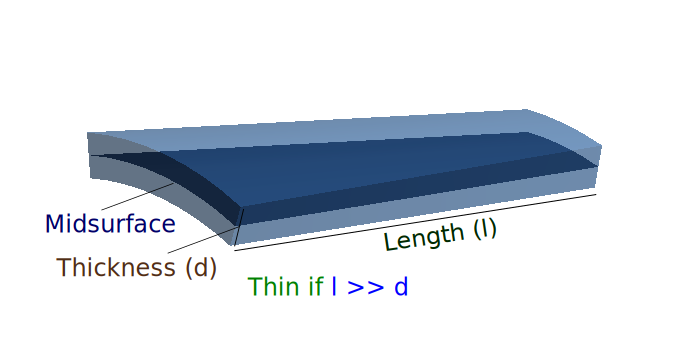
\includegraphics[scale=0.4]{../Common/images//Midsurf.pdf}
	\caption{Midsurface}
	\label{figure_Midsurf}
	\end{figure}

MAT is a locus of the centers of a maximal diameter disc as it rolls around inside the shape. In 2D it is called as 'Midcurve' where as in 3D it is called as 'Midsurface'. Major drawback of this method is that it creates unnecessary branches and is shorter than the corresponding faces on the original solid. Also, slight change in the base geometry forces re-computation resulting in different MAT than the earlier. 

MA creates Midsurface by connecting individual mid-patches generated from 'pairs of surfaces'. This is bettern than MAT as Midsurface is cleaner and abstracts parent shape better; but detecting pairs in complex shapes is difficult and error prone. 

Majority of the above mentioned approaches are based on the final shape and do not use feature information\cite{Smit2011} available in many CAD applications. Another problem is that the Midsurface still lacks exact definition, formalism and algorithms to take care of all practical shapes. This paper proposes use of {\em form features} in formulating Midsurface, in a Generic Programming way.

\subsection{Generic Programming}

Generic Programming is a paradigm of writing algorithms at an abstract level, independent of the form of the data. It reduces repetition and helps in code-reuse, as programmers do not need to write separate implementations for different data structures \cite{Giovannelli2013}. Genesis of Generic Programming can be attributed to David Musser and Alexander Stepanov, in the early 1970s. It became truly popular in 1994 with the advent of Standard Template Library (STL). In STL, algorithms like {\em sort} do not depend directly on containers like {\em list, array}, but on an intermediate entity called {\em Iterator}. As {\em sorting} just needs a way to traverse a collection, it is based on {\em Iterators} only. {\em Iterators} in turn, take care of traversing logic based on the containers \cite{Berti2000}.

Generic Programming has found applications in Geometric Algorithms Libraries like CGAL \cite{Bronnimann}, Boost-Graph, GrAl \cite{Berti2002}.  Algorithms in CGAL are typically parameterized by a {\em traits class}. It encapsulates the basic geometric types (and the operations on them) that are expected by an algorithm. User need not translate-copy his/her data model into data model expected by the algorithm but just has to wrap {\em trait} functionality in terms of own functionality.

Usually, for using an external library or for interoperability between two systems, data from the source system is read, copied into newly instantiated objects of the destination system, so that destination algorithms work on them. In the Generic Programming paradigm, no copy is made. Algorithms are written in a generic way, they are based on few predicates, if these predicates are provided by the source system, then source data can be used as is. {\em Traits} are used to consolidate the predicates that, depending upon a type have slight variations in terms of structure and/or behavior. To achieve this end, {\em Traits} rely on explicit template specialization.  This feature allows you to provide a separate implementation of a class template for a specific type.
